\documentclass[12pt, a4 paper]{article}
% Set target color model to RGB
\usepackage[inner=2.0cm,outer=2.0cm,top=2.5cm,bottom=2.5cm]{geometry}
\usepackage{setspace}
\usepackage[rgb]{xcolor}
\usepackage{environ}
\usepackage{verbatim}
\usepackage{subcaption}
\usepackage{outlines}
\usepackage{enumitem}
\usepackage{amsgen,amsmath,amstext,amsbsy,amsopn,tikz,amssymb,tkz-linknodes}
\usepackage{fancyhdr}
\usepackage{pgfplots}
\usepackage{mathtools}
\usepackage[colorlinks=true, urlcolor=blue,  linkcolor=blue, citecolor=blue]{hyperref}
\usepackage[colorinlistoftodos]{todonotes}
\usepackage{rotating}

\linespread{1.6} % Double Line Spacing
\usetikzlibrary{arrows.meta,intersections,calc}

\hypersetup{%
pdfauthor={Vignesh Ravibaskar},%
pdfcreator={PDFLaTeX},%
pdfproducer={PDFLaTeX},%
}

% Our custom enumerate labelling, just making the outlines bold basically
\setlist[enumerate,1]{label=\textbf{\arabic*}}
\setlist[enumerate,2]{label=\textbf{({\alph*})}}
\setlist[enumerate,3]{label=\textbf{({\roman*})}}

\title{Differentiation}
\author{Derek, Vignesh}
\date{2020}

\newcommand{\comm}[1]{}
\NewEnviron{answer}{\vspace{3mm} \\ \color{blue} {\BODY} \color{black}}
%\NewEnviron{answer}{\color{blue} \comm{\BODY} \color{black}} % Use this method to hide all answers

\begin{document}

\maketitle

\textbf{DIFFERENTIATION [TBC Marks]}
\begin{outline}[enumerate]

\1 Differentiate with respect to $x$ the following: %Question 1

	\2 $\ln (\ln ({x^2}))$\hfill[2]

	\2 $4^{\cos 4x}$\hfill[2]

	\2 $\tan ^{ - 1}(xy)$\hfill[2]

	\2 $\dfrac{{{x^2}}}{3} - \dfrac{{{y^2}}}{4} = 1$\hfill[2]

\1 Solve the following differential equations: %Question 2

	\2 $\dfrac{{{\rm{d}}y}}{{{\rm{d}}x}} = 2y,\;y = 1{\textrm{ when }}\,x = 1$ \hfill[2]

	\2 $\dfrac{{{\rm{d}}x}}{{{\rm{d}}t}} = 4({x^2} + x + 1)$ \hfill[3]

	\2 $\dfrac{{{\rm{d}}y}}{{{\rm{d}}x}} = \dfrac{{ - {e^{ - 3x}}}}{{3y}}$ \hfill[3]

\1 The parametric equations of curve C are: \[x = t + 1,\;y = \frac{1}{{{t^2} + 2t + 2}}{\textrm{ where }} - 3 \leq t \leq 1.\] %Question 3

	\2 Find the Cartesian equation of $C$. \hfill[2]

	\2 Find the equation of the tangent to the curve $C$ when $t=2$.\hfill[3]

\1 Two variables $x$ and $y$ vary with time $t$ in minutes and are connected by the equation $\sin (xy) = \frac{1}{2}$. Given that $x$ increases at a rate of 3 units per minute, find the rate of decrease of $y$ when $y = 1$. \hfill[5] %Question 4

\1 The parametric equations of curve C are: \[x = 1 + {e^{ - at}},\;y = {e^{at}} + {e^{ - at}}\;{\textrm{ where }}t \geq 0.\] %Question 5

	\2  Sketch $C$, including all stationary points and asymptotes where applicable.\hfill[2]

	\2 Find the equation of the normal to the curve $C$ at $t = \frac{\ln{2}}{{2a}}$.\hfill[3]

	\2 What can be said about the normals to the curve $C$ as $t$ gets large?\hfill[1]

\1 A boy throws a rock in the air. It is launched at an angle $\theta$ to the horizontal ground, where $0 < \theta  < \frac{\pi }{2}$. As shown in the diagram, its position in the air $(x,y)$, where $x$ is the horizontal position and $y$ is the vertical position, is approximated by: \[x = (20\cos \theta )t,\,\;y = (20\sin \theta )t - 5{t^2},\]where $t$ is the time in seconds.\\
\[
\begin{tikzpicture}
 \begin{axis}[
	 axis lines = center,
	 xlabel = $x$,
	 ylabel = $y$,
	 xmin = 0, xmax=4.5,
	 ymin = 0, ymax=4.5,
	 xticklabels = {,,},
	 yticklabels = {,,},
	 legend pos=north east
	]
	\addplot [
	 domain=0:3,
	 samples=100,
	 color=blue,
	]
	{x-0.2*x^2};
	\node[label] at (axis cs:0.5,0.23) {$\theta$};
	\addlegendentry{Path of stone};
 \end{axis}
 \draw[->,very thick] (0,0) -- (2,2);
 \draw[thick] (0:0.5) arc (0.5:45:0.5);
\end{tikzpicture}
\]

	\2 Find, in terms of $\theta$,

		\3 The time taken for the toy plane to hit the ground;\hfill[2]

		\3 The maximum height reached by the toy plane;\hfill[2]

		\3 The horizontal distance travelled by the toy plane.\hfill[2]

	\2 Find the angle $\theta$ at which the toy plane should be thrown to attain the maximum horizontal distance.\hfill[2]

\1 A hopper in a butter processing factory is used to store pre-processed butter before it is discharged to the next stage of the manufacturing process. One such hopper is designed with the dimensions as follows:\\
\[
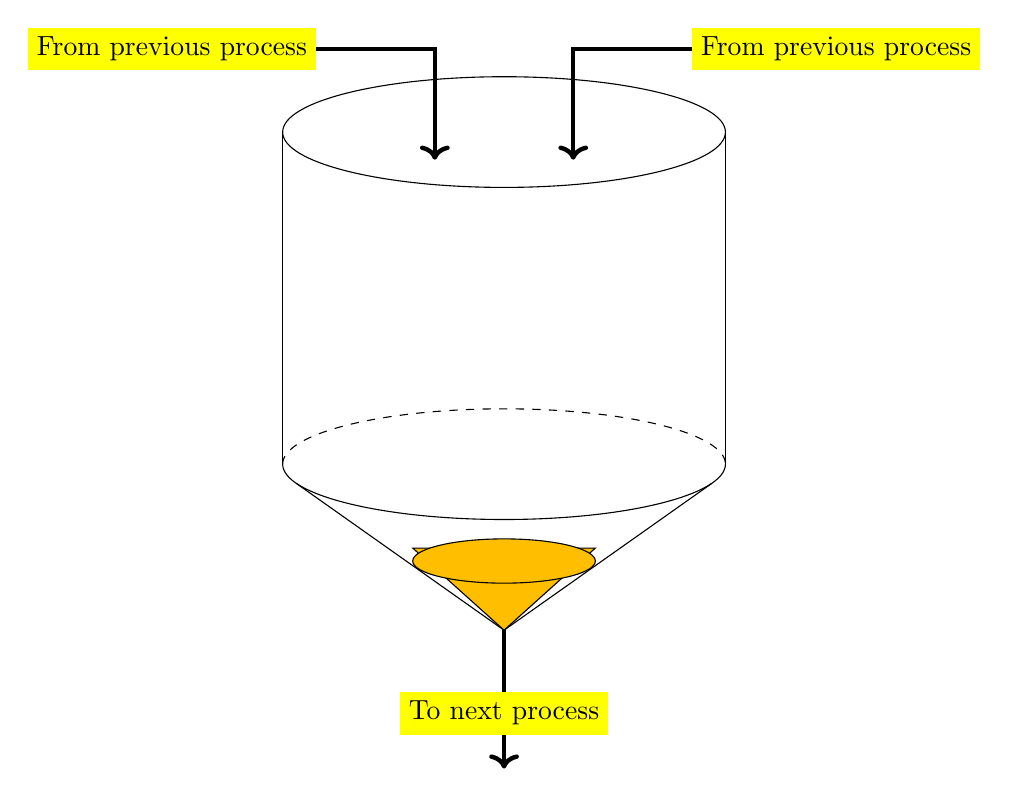
\begin{tikzpicture}
    \draw (0,0) ellipse (80pt and 20pt); %Begin Cylinder
		\draw (-80pt,0) -- (-80pt,-120pt);
		\draw (80pt,0) -- (80pt,-120pt);
		\draw (-80pt,0) -- (-80pt,-120pt);
		\draw[dashed] (-80pt,-120pt) arc (180:0:80pt and 20pt);
		\draw (-80pt,-120pt) arc (180:360:80pt and 20pt); %End Cylinder
		\draw (-75pt,-127pt) -- (0, -180pt); %Begin Cone
		\draw (0,-180pt) -- (75pt,-127pt); %End Cone
		\draw[->,ultra thick] (-120pt,30pt) node [fill=yellow]{From previous process}-- (-25pt,30pt) -- (-25pt,-10pt); %Begin Butter Line
		\draw[->,ultra thick] (120pt,30pt) node [fill=yellow]{From previous process}-- (25pt,30pt) -- (25pt,-10pt);
		\draw[->,ultra thick] (0,-180pt) -- (0,-210pt) node[fill=yellow]{To next process} -- (0,-230pt); %End Butter Line
		\filldraw [orange!50!yellow,draw=black](0,-180pt) -- (33pt,-150.32pt) -- (-33pt,-150.32pt) -- cycle; %Filled Butter
		\filldraw [orange!50!yellow,draw=black](0,-155pt) ellipse (33pt and 8pt);
\end{tikzpicture}
\]


\end{outline}

\end{document}
